% Chapter 5: Design Ideation, Playtesting And Final Product
\chapter{Design Ideation, Playtesting And Final Product}\doublespacing
\label{Chapter5}
\lhead{Chapter V. \emph{Ideation \& Playtesting}}



\section{Game Concept}

Each subsection below corresponds to one working system in the digital prototype and one CSV in its data layer, and is written to carry directly into the physical version: the numbers and structures described here are not proposals, they are the actual configuration already validated in code and playable today.

\subsection{Concept Generation}

The concept was not sketched and then coded --- it was built the other way around. Chapter 3's Design Strategy Statement ("How might we give IITK undergraduates a low-stakes way to rehearse the trade-offs of their four-year lifecycle\dots{}") was answered first as a \textbf{numerically validated digital simulation}, so that the economy --- Time Block costs, SPI thresholds, placement eligibility --- could be tuned and sanity-checked before a single physical component was designed. This is the reverse of the typical board-game process (paper prototype $\rightarrow$ playtest $\rightarrow$ digitize), and is the direct justification for the Chapter 2.7 argument that a digital-first pipeline was the right choice for a project this data-heavy.

\emph{\[ADD: your actual concept-generation narrative --- early sketches, alternative concepts considered and rejected, and why this specific framing (a 4-player rehearsal simulation rather than, say, a single-player app or a facilitated workshop) won out. This is the one part of Chapter 5 that lives only in your own process notes, not in the codebase.\]}

\subsection{Time Management (Time Blocks)}

Every semester allocates exactly 17 Time Blocks (GAME\emph{CONFIG.TIME}BLOCKS\emph{PER}SEMESTER) --- the single currency every other system in the game draws from. Three of the eleven turns (the Interlude, Summer, and Placement turns) allocate zero Time Blocks; they are narrative decision points rather than open action windows, discussed further in 5.2.1. Every action available in a normal turn --- visiting a location, drafting a Project/POR/Internship card, maintaining a social contact --- is priced in Time Blocks first and other resources second, so "how will I spend my week" is always the player's first-order question, directly enacting the balancing-difficulty finding from Chapter 3 (77.2\% agreement) as a mechanic rather than a theme.

Time spending has a second-order consequence through the Burnout Rule: any action whose Stress cost would push total Stress above 10 is blocked outright until the player relieves Stress first (typically by resting or through a social/friction reward). Combined with the Debt Cascade --- any negative Health, Money, or Social value converts 1:1 into Stress before being clamped to zero --- this means Time Blocks are never spent in isolation from wellbeing: an academically aggressive week that ignores Health or Social is quietly building a Stress bill that eventually has to be paid, whether the player notices or not. A separate, unconditional Semester Recovery fires automatically at turns 3, 6, and 9 (+4 Money, +3 Health, âˆ'4 Stress) --- the one restorative mechanic that costs no Time Blocks at all, giving every player a fixed floor of relief regardless of strategy.

\subsection{Academics & Performance (Performance Thresholds)}

Study points accumulate only from a specific subset of Action-phase locations (LHC, NCL, Project Lab, PKK Library, Lab Session, Core Dept Building) --- no other card type in the game rewards Study. At each of the eight academic checkpoints (turns 1, 2, 3, 4, 6, 7, 9, 11), Logic.calculateSemesterSPI converts that semester's accumulated Study into an SPI using the stepped GAME\emph{CONFIG.SPI}GRADING_SCALE (Table 5.1), then resets Study to zero for the next semester. CPI is the running average of every recorded SPI (Logic.updateCPI) --- and at the Summer checkpoint (turn 8), that CPI is permanently locked (state.stats.lockedCPI) based on the first six semesters' transcript. This is Chapter 1's Universal Gates concept implemented exactly as literally as code allows: a single value, fixed at a specific turn, that everything downstream (Section 5.1.7) must be evaluated against, with no way to retroactively improve it.

% Table row: | \textbf{Study Points Required} | \textbf{SPI Awarded} |
% Table row: | ------------------------- | --------------- |
% Table row: | 112                       | 10.00           |
% Table row: | 98                        | 9.00            |
% Table row: | 84                        | 8.00            |
% Table row: | 70                        | 7.00            |
% Table row: | 56                        | 6.00            |
% Table row: | 42                        | 5.00            |
% Table row: | 0 (baseline)              | 4.00            |

\emph{Table 5.1 --- GAME}CONFIG.SPI\emph{GRADING}SCALE_

\subsection{Social Life & Wellbeing}

Health, Stress, and Social are clamped to a 0--10 range every turn (Logic.clampStats), with the Debt Cascade and Burnout Rule described in 5.1.2 acting as the two hard constraints on this triangle. A third, quieter system --- Organic Social Encounters --- ties wellbeing directly to place rather than to random chance: revisiting the same location a set number of times (Visits_Needed in social.csv) deterministically unlocks a named contact tied to that location (e.g., four visits to PKK Library unlocks the Research Professor; two visits to the Hostel Wing unlocks a Wingmate). This directly encodes Chapter 3's Finding 2 --- that support in the real IITK lifecycle forms through repeated informal proximity (wing, canteen, library) rather than a formal matching process --- as a deterministic game rule rather than a random one.

\subsection{Clubs, Sports & PORs}

POR.csv contains 60 cards spanning 15 distinct club/committee "tracks" (e.g. Gymkhana, E-Cell, Election Commission, CWC, Antaragni, Techkriti, Udghosh, Vox Populi), each structured as a 3--4 tier prerequisite chain --- Volunteer $\rightarrow$ Secretary $\rightarrow$ Coordinator/Organiser $\rightarrow$ Head/Fest Coordinator/OC --- with Time cost escalating from 1 block at the entry tier to 4--5 blocks at the top, and each tier requiring the previous one already owned (Req\emph{Prerequisite). One track raises the bar further: the top Gymkhana tier (president}gymkhana) requires both the prior tier card and Social $\geq$ 8, combining a card-prerequisite gate with a stat-threshold gate in a single requirement --- a concrete example of the "Interesting Player Choice" Chapter 4 describes, since no amount of spare Time Blocks alone can buy that position without sustained Social investment elsewhere.

\subsection{Projects, Research & Internships}

projects.csv holds 9 cards (Coding, Algorithms, Research, Design, Hardware, AI, Product, and Academic categories) costing 2--5 Time Blocks each and rewarding only Algo/Research/Product resume points --- never Study. Because Projects and Academics draw from the identical Time Block pool but build entirely separate outcome currencies (resume stats vs. SPI), every block spent on a Project is a block explicitly not spent moving CPI --- the same tension Section 5.5's balancing simulation quantifies directly. internships.csv splits 10 cards between SPO internships (7, summer-only, drafted at the Interlude) and Off-Campus internships (3, semester-long: research, startup-founder, and public-policy tracks), each gated by compound stat thresholds --- the steepest being quant_intern at Algo $\geq$ 3 + CPI $\geq$ 8.5, which foreshadows the equally steep God-Tier Quant placement tier in 5.1.7.

\subsection{Placement & Career Outcomes (Universal Gates)}

placement.csv defines 8 companies ranging from Baseline Safe Placement (CPI $\geq$ 6.5, Algo $\geq$ 1, any internship --- 12--15 LPA) to God-Tier Quant (CPI $\geq$ 9.0, Algo $\geq$ 3, Research $\geq$ 2, and specifically the quant_intern internship card --- 90+ LPA). Logic.evaluateAllPlacements computes a partial match percentage for every company, even ineligible ones, so a player always sees exactly how close they came rather than a flat pass/fail; Logic.getBestPlacementOffer then selects the highest-CTC company among only the fully eligible ones. Because CPI is locked two full turns earlier (5.1.3), this phase is where the consequences of every prior semester's Study/Project/POR balance become irreversible and visible at once --- the clearest single moment in the game where Chapter 1's Universal Gates concept is directly experienced by the player.

\subsection{Random / Friction Events}

friction.csv contains 15 unavoidable events (5 Social, 5 Academic, 2 Health, 3 general-Friction), drawn automatically once per turn (Logic.drawRandomFriction, filtered to the current semester's valid range) and resolved through the same processCardEffect pipeline as any chosen action. Effects range from pure upside (Library Eureka: no cost, +5 Study, âˆ'1 Stress) to pure downside (Surprise Quiz: âˆ'2 Stress with no offsetting reward) to cost-for-benefit trades (Movie Night: 1 Time Block for +1 Social, âˆ'1 Stress) --- variance is not uniformly punishing, but it is uniformly mandatory, which is the actual design lever discussed further under Chapter 4.5. Every card's Flavor_Text is anchored in specific, named IITK geography (MT, PKK Library, the Hall Canteen, LHC), continuing the same grounded voice already present in timeline.csv (Section 5.2.1) rather than introducing a separate, more generic tone for random events.

\subsection{Network & Mentorship}

social.csv defines 8 relationship archetypes (Hostel Wingmate, Helpful Batchmate, Department Senior, Jugaad Friend, Research Professor, Teaching Assistant, Gymkhana Mentor, Industry Mentor), each unlocked deterministically through repeated location visits rather than randomly or by direct purchase (5.1.4). Every contact offers two distinct kinds of value: a repeatable passive reward, claimed each semester by spending Time Blocks on maintenance (Logic.applyMaintenanceRewards), and a separate one-time-only career bonus (Algo/POR/Research/Product), tracked in state.mentorBonusesClaimed so it cannot be re-farmed. This mirrors how most real mentor relationships work --- ongoing informal support plus, at most, one or two genuinely high-leverage favors (a referral, a recommendation letter) rather than an unlimited resource.

\section{Ideation}

\subsection{Phased Gameplay}

The full 11-turn arc (Table/Figure 5.3) was written before it was coded --- timeline.csv already carries a named psychological phase, an "IITK stuff" grounding paragraph, and an original verse for every turn, all authored as part of this project. Three turns break the normal pattern entirely: the Interlude (turn 5, the Comparison Trap --- SPO internship shortlisting), Summer (turn 8, the Trial Run of Adulthood --- the CPI-locking checkpoint), and Placement (turn 10, the Final Verdict) all allocate zero ordinary Time Blocks and instead present a single high-stakes narrative decision, functioning as pacing beats that separate the eight "normal" resource-management turns into three acts.

\begin{figure}[h]
\centering
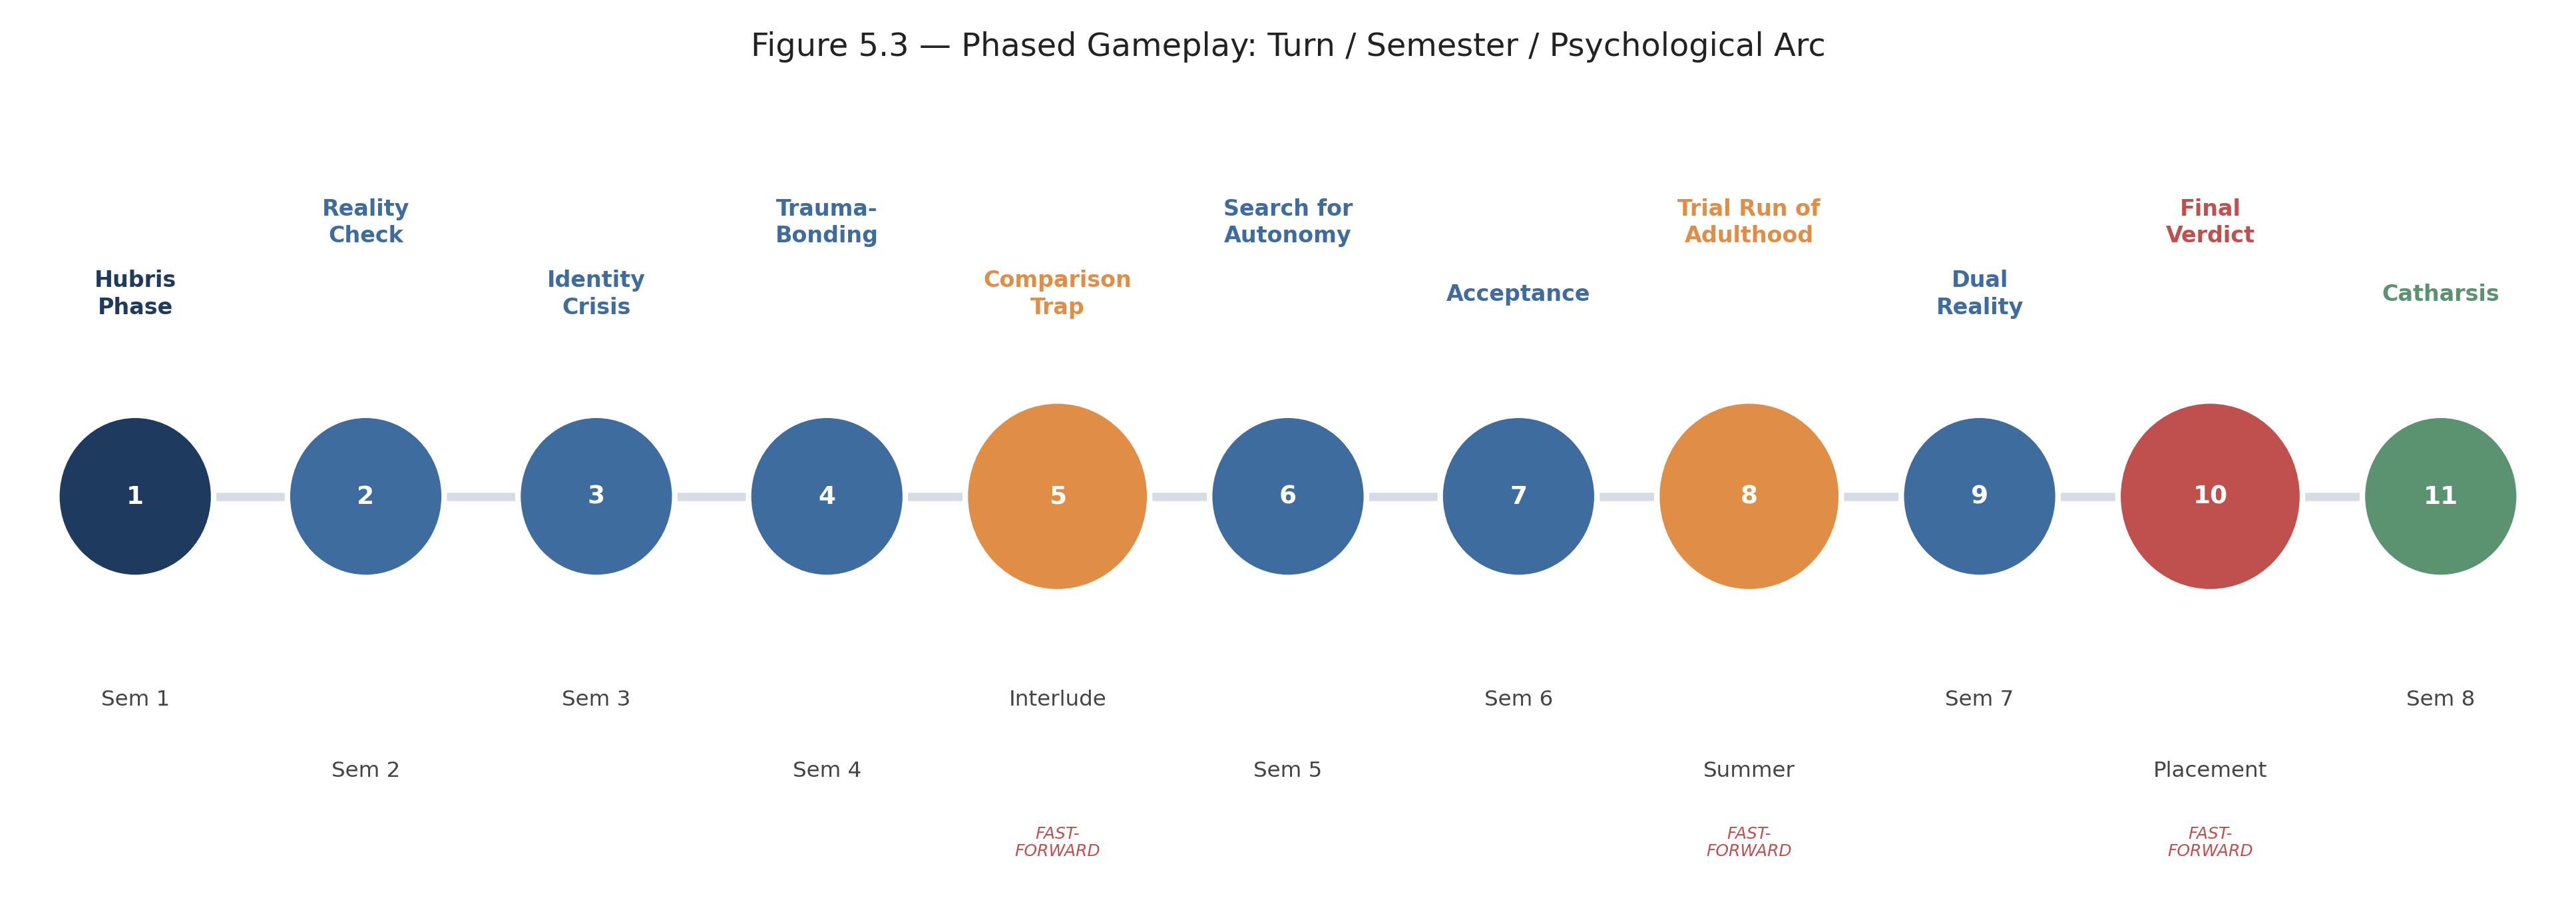
\includegraphics[width=0.8\textwidth]{Pictures/fig_5_1.png}
\caption{Figure 1 from Chapter 5}
\end{figure}

\emph{Figure 5.3 --- Phased Gameplay: Turn / Semester / Psychological Arc (from timeline.csv)}

The arc's own language is worth preserving directly: Semester 1 opens as \emph{"The Hubris Phase"} --- arriving "carrying the weight of being a topper" --- and by Semester 2 gives way to \emph{"Cognitive Dissonance"}, where, in the file's own words, \emph{"hard work does not guarantee an 'A' grade anymore."} This is not decorative flavor text sitting on top of the mechanics; it is the same design document as the mechanics --- the Reality Check phase (turn 2) is precisely when the SPI\emph{GRADING}SCALE first resolves a semester's Study investment into a number the player cannot argue with.

\subsection{Emergent Gameplay}

\begin{itemize}\item Compounding bad semesters: Stress from an unlucky Friction draw stacks with Stress from Debt Cascade (a Health or Money shortfall converting 1:1), which can trigger the Burnout Rule and block a planned high-value action --- a single rough week can cost a player more than the week itself.\item Track lock-in: POR tiers are both prerequisite-gated and semester-windowed (Sem\emph{End), so a track not started early enough cannot be caught up on later purely by spending more Time Blocks --- e.g. president}gymkhana (Sem_End = 8, requires the prior tier and Social $\geq$ 8) is simply unreachable for a player who starts the Gymkhana track in Semester 6.\item Divergent end-states from identical spend: because Study and resume stats (Algo/Res/Prod/POR) are earned from entirely non-overlapping cards, two players who spend the same total number of Time Blocks across the game can end up with completely different profiles --- one high-CPI/low-resume, one low-CPI/high-resume --- purely from allocation choices. Section 5.5 measures exactly how sharply this diverges.\item Emergent "home base" behavior: because Organic Social Encounters reward repeat visits to the same location rather than chasing novelty, players who lean into wellbeing tend to converge on 2--3 "home" locations rather than spreading visits thin --- an unplanned but thematically appropriate echo of Chapter 3's wing-centric reliance finding.\end{itemize}

\section{Playtesting}

\emph{This section has not been run yet --- it needs real 4-player sessions, not simulated ones. What follows is a ready-to-execute plan, not a report; replace the bracketed placeholders below with what actually happens once you run it.}

Recruitment: your Chapter 3 survey already produced a usable pool --- 58 of 113 respondents who answered the consent question (51.3\%) indicated willingness to be recontacted for playtesting. That is a large enough pool to comfortably fill 3--4 tables of 4 players each, drawn from a population that already understands the problem space the game addresses, without needing fresh recruitment.

\textbf{\emph{5.3.1 Methods Of Playtesting}}

\begin{itemize}\item Format: in-person, 4 players per table, matching the final product's player count exactly (a remote/digital playtest of the browser prototype could supplement this but should not replace an in-person physical-component test).\item Target: at minimum 2--3 full playthroughs (full 11-turn arc) with distinct groups, to separate genuine design issues from one group's idiosyncrasies.\item Instrumentation: a facilitator observation log (confusion points, house-ruling, turns where players stalled), a lightweight think-aloud prompt during the Placement turn specifically (since it is the highest-stakes single moment), and a short post-session questionnaire reusing a subset of your Chapter 3 Likert items (clarity, overwhelm, perceived fairness) so playtesting results are directly comparable to your survey baseline.\end{itemize}

\emph{\[ADD once run: exact dates, locations, number of sessions, and participant composition (Year/Branch mix, ideally including some of the same personas from Chapter 3.6).\]}

\textbf{\emph{5.3.2 Outcomes From Playtesting}}

\emph{\[ADD once run: what worked, what confused players, which mechanic needed the most facilitator intervention, and how session length compared to expectations.\]}

\textbf{\emph{5.3.3 Game Concept Tuning}}

\emph{\[ADD once run: concrete rule/number changes made in response to 5.3.2, with before/after values --- this is also where any Chapter 4 open decisions (Victory Conditions especially) should be confirmed against real player reactions rather than left as design-time proposals.\]}

\section{Final Product}

\subsection{Product Intro}

The final product is \emph{\[GAME NAME\]}, a 4-player physical board game adapting the validated digital economy described in Section 5.1 into a tabletop format. Every number quoted in this chapter --- Time Block costs, SPI thresholds, placement requirements --- carries forward unchanged from the working prototype; what remains to design is the physical form those numbers take.

\subsection{Game Components}

Proposed component list, derived directly from the CSV structure above (cross-check against your Chapter 4, Section 4.4.2 answer and reconcile any differences before finalizing):

\begin{itemize}\item 1 shared board --- 20 Action-phase locations (locations.csv), likely organized by Zone (Academic / Hostel / Social / Health / Career) rather than a linear path\item Project deck --- 9 cards\item POR deck --- 60 cards across 15 tracks (consider whether all 15 tracks belong in a physical deck, or whether a curated subset per playtest keeps table time reasonable --- flag as an open decision for 5.3.3)\item Internship deck --- 10 cards (7 SPO / 3 Off-Campus)\item Placement deck --- 8 cards, revealed only at the Placement turn\item Friction/Event deck --- 15 cards, shuffled and drawn once per turn\item Social/Network deck or tracker --- 8 contact cards, or a shared board track given they unlock deterministically rather than by draw\item 4 player mats --- tracking Health / Stress / Social / Money / Study / CPI / resume stats per player\item Time Block tokens (17 per player per semester) and resource tokens for the five survival stats\end{itemize}

\subsection{Game Board (4-Player Layout)}

\emph{\[Pending physical design --- headings ready to populate once you have a layout.\]}

\subsection{Player Mat / Character Sheet}

\emph{\[Pending physical design.\]}

\subsection{Cards}

\emph{\[Pending physical design --- content/values are already final (Section 5.1); this section needs visual/print design only.\]}

\subsection{Tokens}

\emph{\[Pending physical design.\]}

\subsection{Other Pieces}

\emph{\[Pending physical design.\]}

\subsection{Sequence Of Play}

A normal turn (1, 2, 3, 4, 6, 7, 9, 11) follows a fixed four-phase cycle:

\begin{itemize}\item 1\. Narrative --- the turn's phase and psychology are presented (Section 5.2.1); at turns 3, 6, and 9 the automatic Semester Recovery is also applied here.\item 2\. Friction --- one unavoidable random event is drawn and resolved (Section 5.1.8).\item 3\. Opportunity --- the player may draft one card from the Project, POR, or Off-Campus Internship pools available that semester (Sections 5.1.5--5.1.6).\item 4\. Action --- the player spends any remaining Time Blocks on locations (Section 5.1.4--5.1.5), each visit immediately ending the turn once resolved.\end{itemize}

Turns 5, 8, and 10 replace this cycle with a single narrative decision (Interlude internship shortlist, Summer path choice, Placement resolution) and allocate no ordinary Time Blocks. On academic turns, the Action phase closes with an SPI calculation and report-card reveal (Section 5.1.3) before advancing to the next turn's Narrative phase.

\subsection{Ending The Game}

The game concludes at turn 11 (Semester 8, "Catharsis") immediately following Placement resolution at turn 10. In the current single-player prototype, "ending" means the narrative closes and the best eligible offer (if any) is revealed. For the 4-player physical version, this is the point at which \textbf{Chapter 4's Victory Conditions} (Section 4.3.2) determine how the four players' final states are compared --- this section should be finalized once that decision is confirmed, rather than duplicated here.

\section{Balancing The Game Data}

Table 5.1 (Section 5.1.3) and Table 5.2 below give the core numeric benchmarks already encoded in GAME_CONFIG and the CSVs.

% Table row: | \textbf{Action Type}                                                 | \textbf{Typical Time Cost} | \textbf{Typical Reward}                        |
% Table row: | --------------------------------------------------------------- | --------------------- | ----------------------------------------- |
% Table row: | Academic location visit (LHC / NCL / Project Lab / Lab Session) | 1                     | +14 Study                                 |
% Table row: | Academic location visit (PKK Library)                           | 1 (+1 Study cost)     | +21 Study net +20                         |
% Table row: | Academic location visit (Core Dept Building, Sem 4+)            | 1                     | +21 Study                                 |
% Table row: | POR track, Tier 1 (Volunteer)                                   | 1                     | +0--1 POR                                  |
% Table row: | POR track, Tier 4 (Head / Fest Coordinator)                     | 4--5                   | +2--3 POR (+1 Prod, some tracks)           |
% Table row: | Project card                                                    | 2--5                   | +1--4 Algo / Res / Prod (varies)           |
% Table row: | Social maintenance (per contact, per semester)                  | 0--1                   | stat rewards + one-time career bonus      |
% Table row: | Random Friction event                                           | 0--1 (unavoidable)     | varies --- can be pure cost or pure benefit |

\emph{Table 5.2 --- Representative Time Block costs across systems}

\subsection{Simulated Playthroughs}

To check whether these numbers are balanced against each other, a Monte Carlo simulation was built in Python, re-implementing the exact formulas above (SPI\emph{GRADING}SCALE, the 17-block semester allowance, the Debt Cascade, the Burnout clamp, and the placement eligibility matching from Logic.evaluateAllPlacements) rather than estimating them. Five archetypal play strategies were run for 800 trials each: an \textbf{Academic Maximalist} (heavy Study focus), a \textbf{Balanced Builder} (even spread), a \textbf{POR Climber}, a \textbf{Portfolio Builder} (Project/Internship focus), and a \textbf{Low-Structure} archetype modelling the high-overwhelm, low-clarity behavior pattern from the Chapter 3.6 "Aditi" persona. This is a simplified proxy model --- one representative POR track, an approximated internship-eligibility flag, semesters 1--6 for the CPI lock and semester 7 for late resume-building --- built to check relative balance, not to predict exact play.

\begin{figure}[h]
\centering
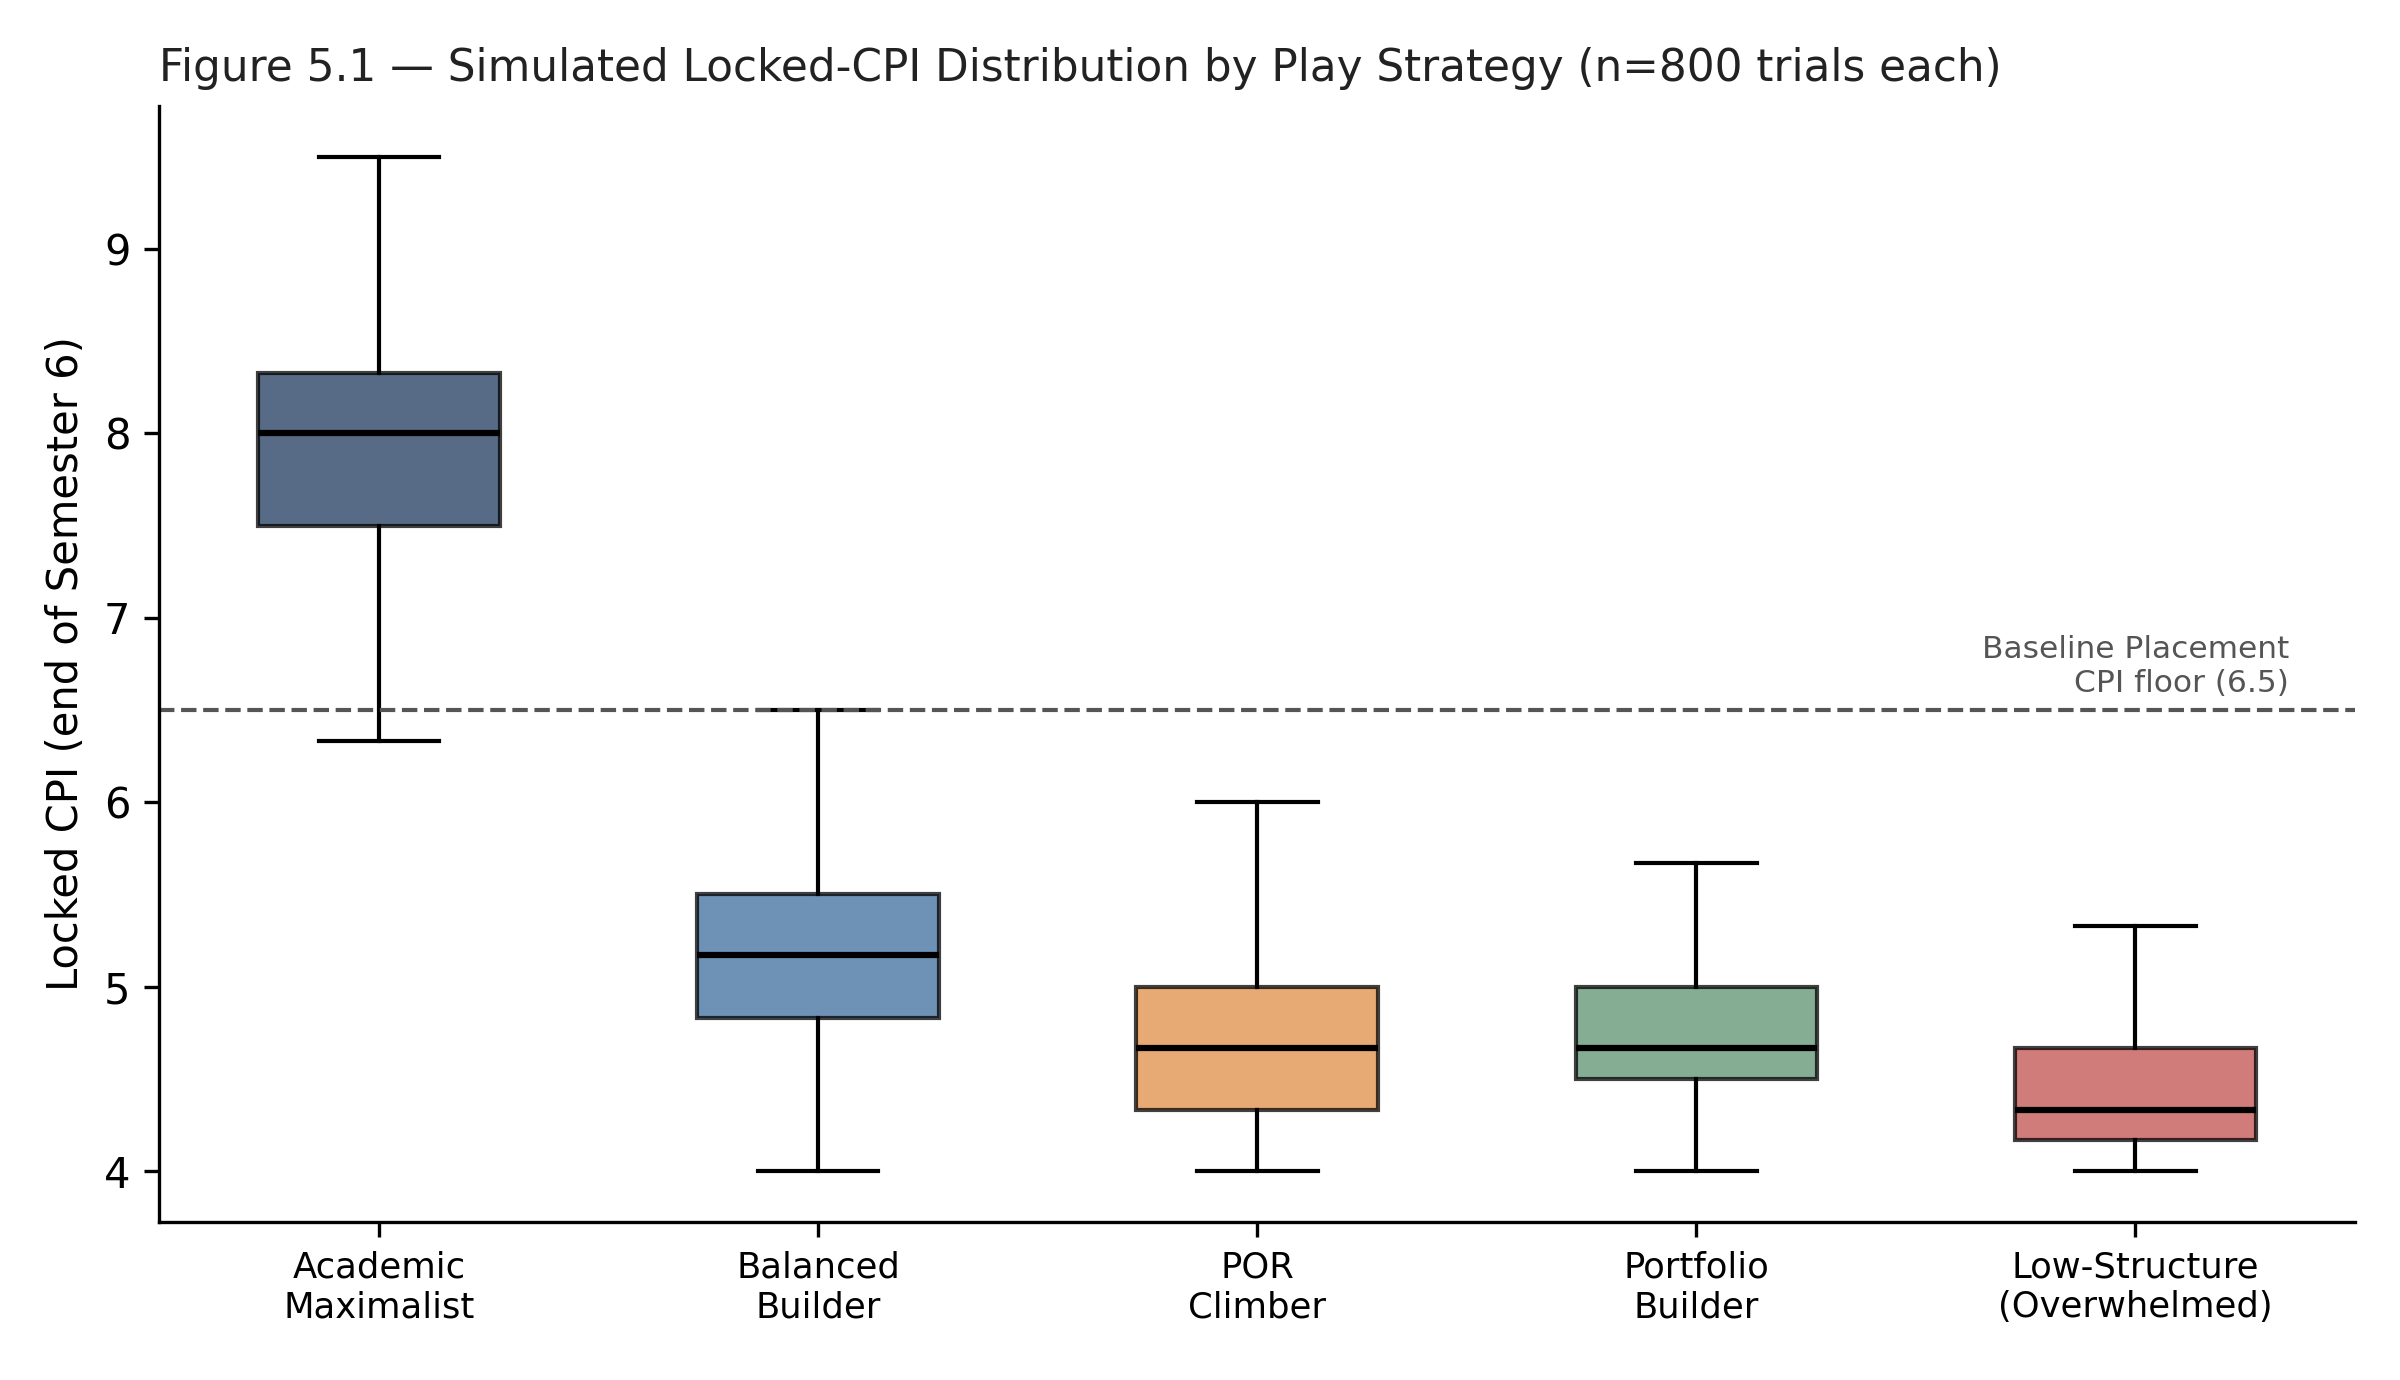
\includegraphics[width=0.8\textwidth]{Pictures/fig_5_2.png}
\caption{Figure 2 from Chapter 5}
\end{figure}

\emph{Figure 5.1 --- Simulated Locked-CPI Distribution by Play Strategy (n = 800 trials each)}

\begin{figure}[h]
\centering
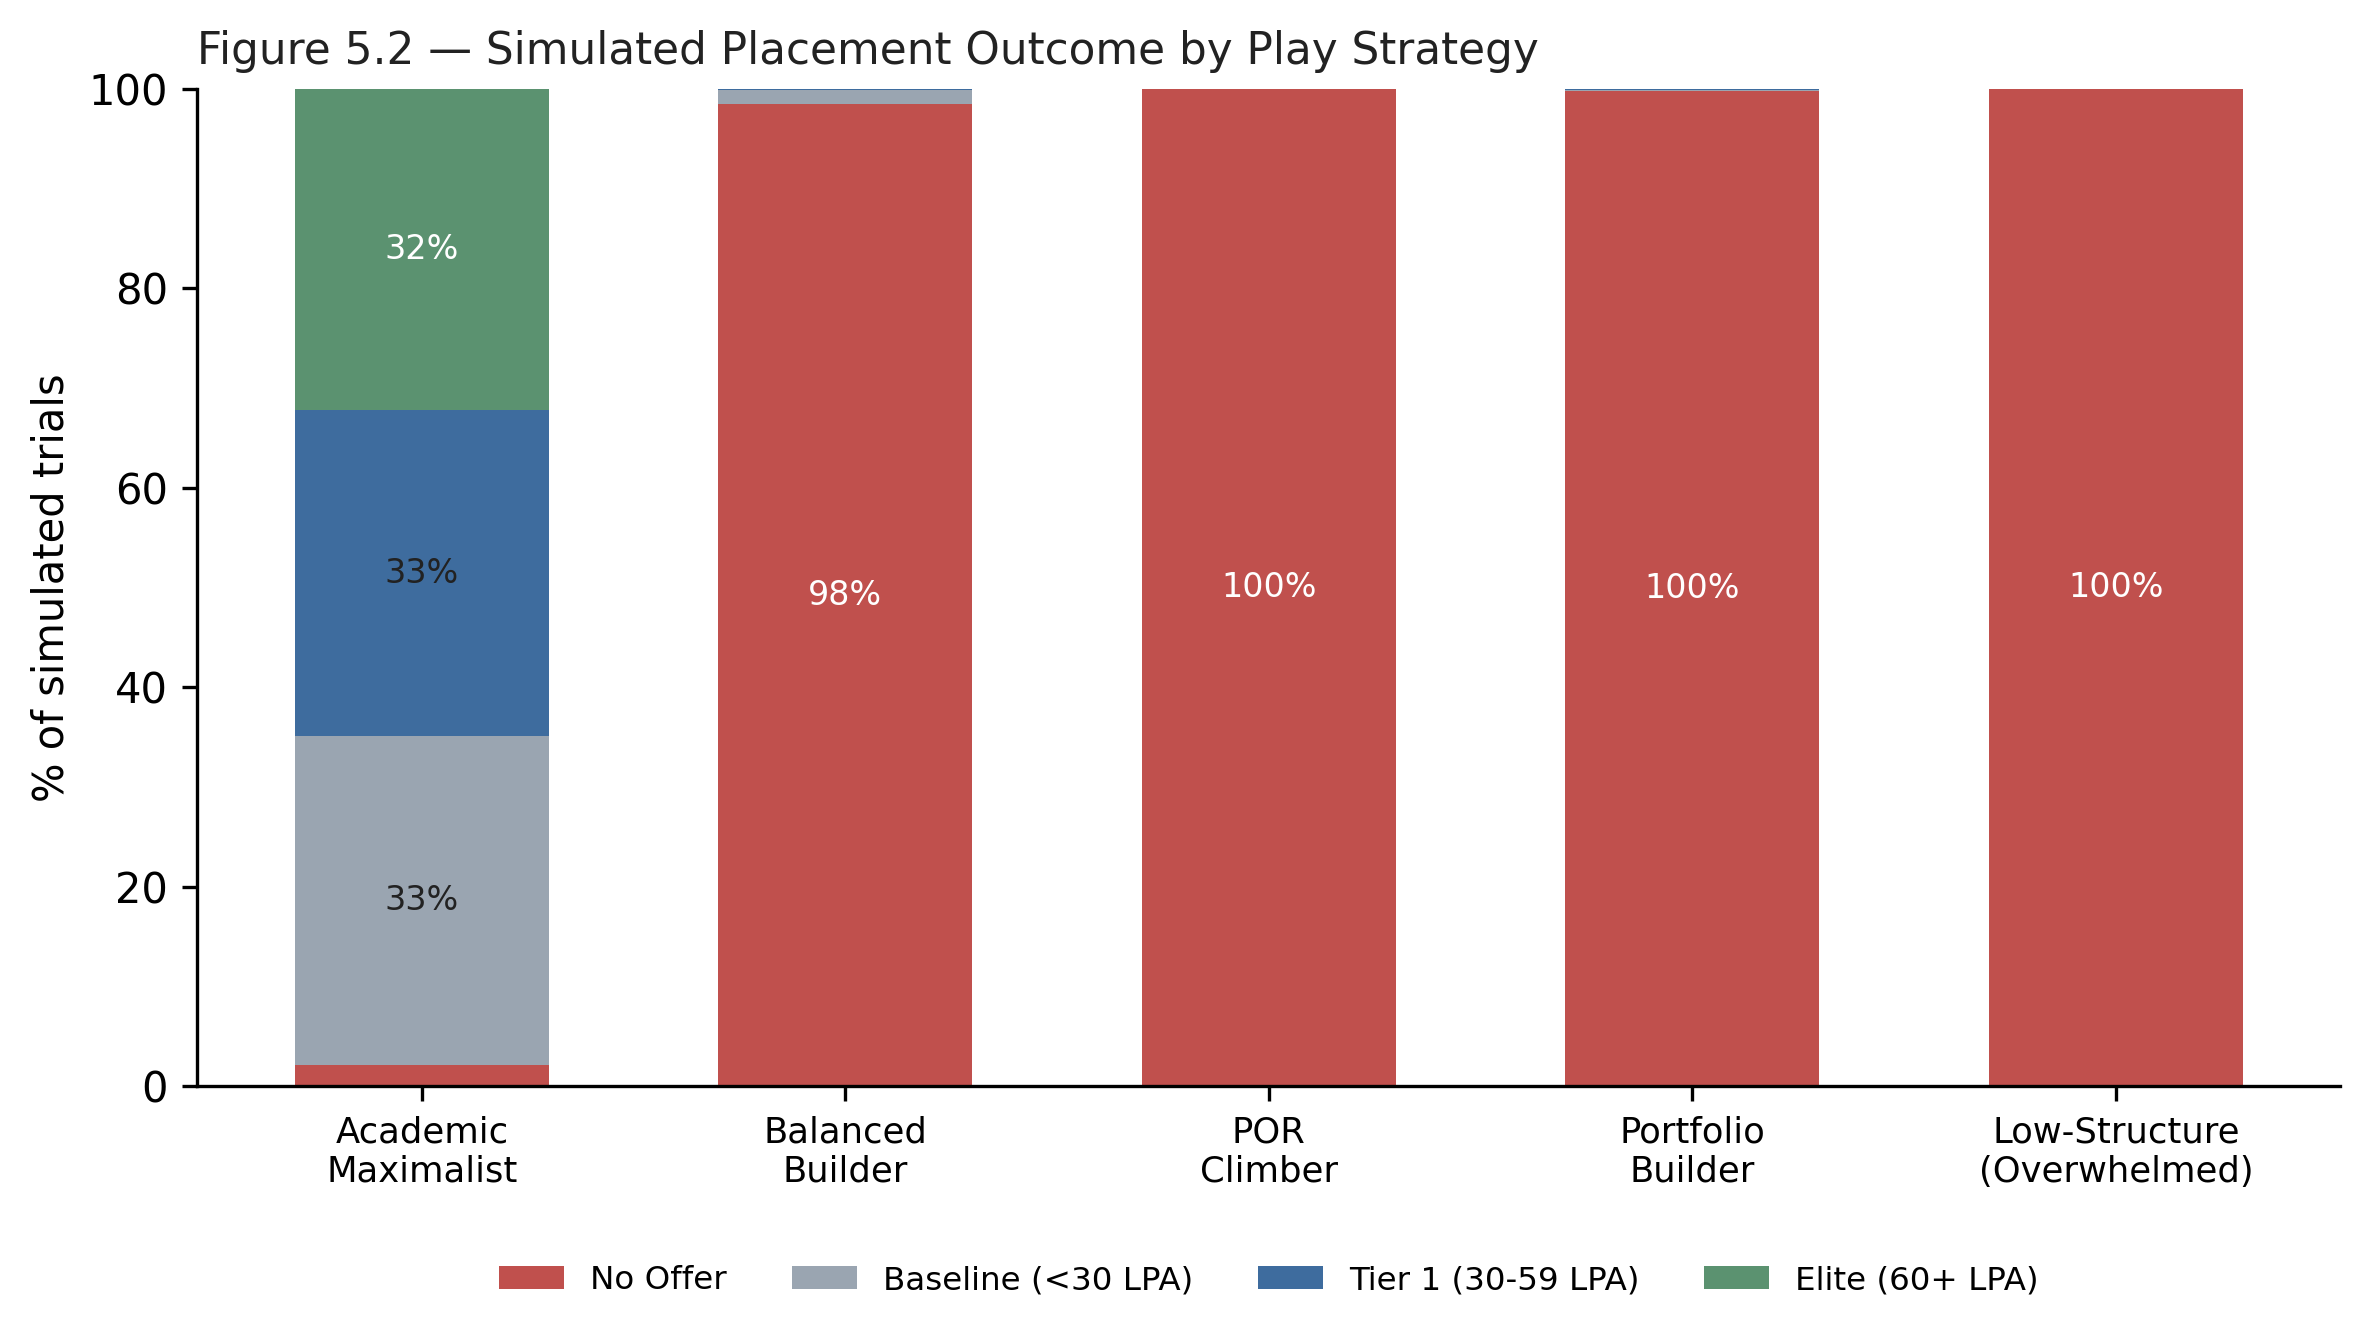
\includegraphics[width=0.8\textwidth]{Pictures/fig_5_3.png}
\caption{Figure 3 from Chapter 5}
\end{figure}

\emph{Figure 5.2 --- Simulated Placement Outcome by Play Strategy}

% Table row: | \textbf{Archetype}               | \textbf{Mean CPI} | \textbf{Median CPI} | \textbf{\% CPI$\geq$8.0} | \textbf{\% CPI<6.5} | \textbf{\% No Offer} | \textbf{Mean CTC (LPA)} |
% Table row: | --------------------------- | ------------ | -------------- | ------------- | ------------- | -------------- | ------------------ |
% Table row: | Academic Maximalist         | 7.92         | 8.00           | 53.1\%         | 1.1\%          | 2.1\%           | 49.4               |
% Table row: | Balanced Builder            | 5.20         | 5.17           | 0.0\%          | 98.5\%         | 98.5\%          | 0.3                |
% Table row: | POR Climber                 | 4.67         | 4.67           | 0.0\%          | 100.0\%        | 100.0\%         | 0.0                |
% Table row: | Portfolio Builder           | 4.75         | 4.67           | 0.0\%          | 99.8\%         | 99.8\%          | 0.1                |
% Table row: | Low-Structure (Overwhelmed) | 4.44         | 4.33           | 0.0\%          | 100.0\%        | 100.0\%         | 0.0                |

\emph{Table 5.3 --- Simulation summary across 5 archetypes Ã--- 800 trials}

\textbf{Finding.} Only the Academic Maximalist archetype reliably clears any placement gate (97.9\% receive an offer, mean CTC ≈₹49.4 LPA); all four other archetypes fail to reach even the Baseline Safe Placement CPI floor (6.5) in 98.5--100\% of trials, because Study --- and therefore SPI and CPI --- is earned exclusively from a small set of Academic locations, while Projects and PORs build entirely separate resume currencies that contribute nothing to CPI. As currently balanced, diversifying away from pure academic focus does not trade off against placement outcome --- it forfeits it almost entirely.

\textbf{This is worth a deliberate decision, not an accidental one.} Three directions are available: (a) lower the baseline CPI floor so a Balanced or Portfolio strategy can still clear it, (b) let select Projects or top-tier PORs grant a small Study side-reward so non-academic investment has some CPI payoff, or (c) keep the numbers as they are, treating the steep CPI gate as an intentional design statement --- a direct, playable echo of Chapter 3's own finding that IITK's system rewards academic focus far out of proportion to how much students say they value it (Section 3.3, Figure 3.11: Career Prep and Health \& Wellness are simultaneously the most wished-for and least-served domains). Whichever direction is chosen, it should be tested explicitly in Section 5.3 playtesting rather than decided from simulation data alone.

\textbf{This finding is not just a game-balance artifact --- it is independently supported by real data.} Section 3.8's decision-tree analysis of 57 real IITK resumes against their actual 2024 placement outcomes shows CPI and Algo_Rigor as the dominant splitting features across nearly every branch, with lower-CPI/lower-Algo profiles routed toward a narrower set of outcomes regardless of their POR, Research, or Product scores. The placement.csv thresholds this simulation tests were themselves informed by that same analysis (Section 3.8), so the sharp Academic-Maximalist-only result above is not an accident of arbitrary game numbers --- it is the game reproducing a pattern that is already present in real IITK placement data, which strengthens rather than undermines the case for treating it as a deliberate design statement (option (c) above).

\textbf{References}

This list consolidates all citations used across Chapters 1--5 into a single sequence. Reference \[43\] was added during the integration pass to correctly source the emerging-adulthood claim in Section 2.1, which previously pointed to an unrelated source (see the audit note at the end of this section).

\textbf{\[1\]} Lisa K. Simon. 2025. Is AI responsible for the rise in entry-level unemployment? Revelio Labs Macro News. Retrieved May 30, 2026 from <https://www.reveliolabs.com/news/macro/is-ai-responsible-for-the-rise-in-entry-level-unemployment/>

\textbf{\[2\]} Theodore Gerard Lynn, Pierangelo Rosati, Edel Conway, and Lisa van der Werff. 2023. The Future of Work: Challenges and Prospects for Organisations, Jobs and Workers. Palgrave Macmillan, Cham, Switzerland. <https://doi.org/10.1007/978-3-031-31494-0>

\textbf{\[3\]} Observer Research Foundation. 2023. Young India and Work: A Survey of Youth Aspirations. ORF Report. Retrieved May 30, 2026 from <https://www.orfonline.org/public/uploads/posts/pdf/20230420163450.pdf>

\textbf{\[4\]} Mercer Mettl. 2025. India's Graduate Skill Index 2025: Talent Readiness of Indian Graduates for an AI-Enabled Workplace. Technical Report. Retrieved May 30, 2026 from <https://www.mercer.com/insights/talent-and-transformation/talent-assessment/indias-graduate-skill-index-2025/>

\textbf{\[5\]} Gakujo Co., Ltd. 2023. Perspectives on Job Hunting: Survey of 2024 Graduates. PR TIMES Research Report. Retrieved May 30, 2026 from <https://service.gakujo.ne.jp/press/230412>

\textbf{\[6\]} Cabinet Office, Government of Japan. 2024. Survey on Student Job-Hunting Schedules and Academic Impact. Cabinet Office Economic and Social Research Institute Report. Retrieved May 30, 2026 from <https://www5.cao.go.jp/keizai1/gakuseichosa/index.html>

\textbf{\[7\]} Ziyi Wang, Ziwen Zeng, Yuan Li, and Zijian Ding. 2025. CareerPooler: AI-Powered Metaphorical Pool Simulation Improves Experience and Outcomes in Career Exploration. arXiv preprint arXiv:2509.11461. <https://doi.org/10.48550/arXiv.2509.11461>

\textbf{\[8\]} Koji Yatani, Zefan Sramek, and Chi-Lan Yang. 2024. AI as Extraherics: Fostering Higher-order Thinking Skills in Human-AI Interaction. arXiv preprint arXiv:2409.09218. <https://doi.org/10.48550/arXiv.2409.09218>

\textbf{\[9\]} Hayeon Jeon, Suhwoo Yoon, Keyeun Lee, et al. 2025. Letters from Future Self: Augmenting the Letter-Exchange Exercise with LLM-based Agents to Enhance Young Adults' Career Exploration. In Proceedings of the 2025 CHI Conference on Human Factors in Computing Systems (CHI '25). ACM, New York, NY, USA, 1--21. <https://doi.org/10.1145/3706598.3714206>

\textbf{\[10\]} Wantong Du, Zhiying Zhu, Xinhui Xu, Haoyuan Che, and Shi Chen. 2024. CareerSim: Gamification Design Leveraging LLMs For Career Development Reflection. In Extended Abstracts of the CHI Conference on Human Factors in Computing Systems (CHI EA '24). ACM, New York, NY, USA, 1--7. <https://doi.org/10.1145/3613905.3650928>

\textbf{\[11\]} Pat Pataranutaporn, Kavin Winson, Peggy Yin, Auttasak Lapapirojn, Pichayoot Ouppaphan, Monchai Lertsutthiwong, Pattie Maes, and Hal Hershfield. 2024. Future You: A Conversation with an AI-Generated Future Self Reduces Anxiety, Negative Emotions, and Increases Future Self-Continuity. arXiv preprint arXiv:2405.12514. <https://doi.org/10.48550/arXiv.2405.12514>

\textbf{\[12\]} Lisa A. Pace, Carmen Bruno, and Jan Oliver Schwarz. 2025. Personas in Scenario Building: Integrating Human-Centred Design Methods in Foresight. Futures 166 (February 2025), Article 103539. <https://doi.org/10.1016/j.futures.2025.103539>

\textbf{\[13\]} Brian J. Taber and Maureen Blankemeyer. 2015. Future Work Self and Career Adaptability in the Prediction of Proactive Career Behaviors. Journal of Vocational Behavior 86 (2015), 20--27.

\textbf{\[14\]} Danqi Wang and Yanling Li. 2024. Career Construction Theory: Tools, Interventions, and Future Trends. Frontiers in Psychology 15 (2024), Article 1381233.

\textbf{\[15\]} Bandura, A. 1986. Social Foundations of Thought and Action: A Social Cognitive Theory. Prentice-Hall.

\textbf{\[16\]} Hackett, G., \& Betz, N. E. 1981. A self-efficacy approach to the career development of women. Journal of Vocational Behavior, 18(3), 326--339. <https://doi.org/10.1016/0001-8791(81)90019-1>

\textbf{\[17\]} Savickas, M. L. 2013. Career construction theory and practice. In S. D. Brown \& R. W. Lent (Eds.), Career Development and Counseling (2nd ed., pp. 147--183). John Wiley \& Sons.

\textbf{\[18\]} Savickas, M. L., \& Porfeli, E. J. 2012. Career Adapt-Abilities Scale: Construction, reliability, and measurement equivalence across 13 countries. Journal of Vocational Behavior, 80(3), 661--673.

\textbf{\[19\]} Low, C. W., Cheng, M. Y., \& Ng, K. Y. 2026. Undergraduates' career adaptability: a systematic review of predictors, mediators, and outcomes. Issues and Perspectives in Business and Social Sciences, 6(2), 340--353. <https://doi.org/10.33093/ipbss.2026.6.2.8>

\textbf{\[20\]} Wang, Y. 2026. The impact of career adapt-abilities on AI anxiety among English majors: a dual perspective analysis based on core self-evaluations at the person- and variable-centered. Frontiers in Psychology, 17, Article 1767791. <https://doi.org/10.3389/fpsyg.2026.1767791>

\textbf{\[21\]} YaÅŸar, H., \& Karagucuk, V. 2025. The effect of artificial intelligence anxiety on career decidedness among students in English-related departments at universities. Discover Artificial Intelligence, 5(1), 48. <https://doi.org/10.1007/s44163-025-00284-y>

\textbf{\[22\]} Carkit, E. 2025. A social cognitive lens on employment anxiety and career optimism in the transition from school to work. The Career Development Quarterly, 73(3), 194--204. <https://doi.org/10.1002/cdq.70000>

\textbf{\[23\]} Zhang, J., Talib, M. A., \& Wang, J. 2025. Enhancing career adaptability and career decision-making self-efficacy through career planning education: a quasi-experimental study. Frontiers in Psychology, 16, 1612768. <https://doi.org/10.3389/fpsyg.2025.1612768>

\textbf{\[24\]} Maji, S., Chaturmohta, A., Deevela, D., Sinha, S., \& Barsaiya, A. 2024. Mental health consequences of academic stress, amotivation, and coaching experience: A study of India's top engineering undergraduates. Psychology in the Schools, 61(9), 3540--3566. <https://doi.org/10.1002/pits.23230>

\textbf{\[25\]} Afreen, \& Alam, S. 2022. Academic stress and suicidal ideation concerning mental health among coaching students preparing for technical entrance exams. International Journal of Multidisciplinary Educational Research, 11(11), 160--168.

\textbf{\[26\]} Chandrasekera, T., Hosseini, Z., Jayadas, A., \& Boorady, L. M. 2024. PeTe (Peer Teaching) Mentors: How Near Peer Mentoring (NPM) Affects Academic Success and Retention in Design Education. Innovative Higher Education, 49(5), 975--991. <https://doi.org/10.1007/s10755-024-09709-5>

\textbf{\[27\]} Yasar, D., \& Küçükali, U. F. 2026. Evaluating a near-peer mentoring model in a vertical studio: a mixed-methods case study with mentee and mentor perspectives. Cogent Education, 13(1), 2696606. <https://doi.org/10.1080/2331186X.2026.2696606>

\textbf{\[28\]} Bayeck, R. Y. 2020. Examining Board Gameplay and Learning: A Multidisciplinary Review of Recent Research. Simulation \& Gaming, 51(4), 411--431. <https://doi.org/10.1177/1046878119901286>

\textbf{\[29\]} Gee, J. P. 2007. What Video Games Have to Teach Us About Learning and Literacy (Revised ed.). Palgrave Macmillan.

\textbf{\[30\]} Gong, H., Bazakidi, E., \& Zary, N. 2019. Serious Games in Health Professions Education: Review of Trends and Learning Efficacy. Yearbook of Medical Informatics, 28(1), 240--248. <https://doi.org/10.1055/s-0039-1677904>

\textbf{\[31\]} Austad, A. F. 1988. Effects of peer mentoring on the achievement and persistence of academically underprepared college freshmen (Doctoral dissertation, University of the Pacific). <https://scholarlycommons.pacific.edu/uop_etds/504>

\textbf{\[32\]} Main, S., \& O'Rourke, J. 2011. 'New Directions for Traditional Lessons': Can Handheld Game Consoles Enhance Mental Mathematics Skills? Australian Journal of Teacher Education, 36(2), 43--55. <https://doi.org/10.14221/ajte.2011v36n2.4>

\textbf{\[33\]} Main, S., \& O'Rourke, J. 2017. Technology in the Classroom: Improving Automaticity in Mental-maths in Primary-aged Students. Australian Journal of Teacher Education, 42(10), 50--70. <https://doi.org/10.14221/ajte.2017v42n10.4>

\textbf{\[34\]} Sousa, M. 2021. City-building board games as systemic educational materials: an analysis of city-building board games. Urban Science, 5(3), 87. <https://doi.org/10.3390/urbansci5030087>

\textbf{\[35\]} Success Print Typographies \& Design Studio. 2024. Inspirational Board Game and Office Typographies. Etsy Shop Archive: Succation.

\textbf{\[36\]} Dhar, U., et al. 2022. Townshipâ„¢ as an empirical platform for resource scheduling. In Simulation and Gaming. ISAGA 2021, LNCS 13219, pp. 3--14. Springer. <https://doi.org/10.1007/978-3-031-09959-5_1>

\textbf{\[37\]} Bartolucci, M., Sparrow, L., \& Freeman, S. O. 2019. Tactile interaction and cognitive mapping in board game play. Journal of Educational Technology Systems, 48(1), 58--75. <https://doi.org/10.1177/0047239519854045>

\textbf{\[38\]} Booth, P. 2019. Board Gamers as Consumer-Fans: Sociality, Association, and Co-Presence in Analogue Play. Games and Culture, 16(2), 154--172. <https://doi.org/10.1177/1555412019890419>

\textbf{\[39\]} Pixelixe Design Blog. 2024. Exploring the role of print in modern digital design studios. Pixelixe Creatives.

\textbf{\[40\]} Carr, N. 2013, February 20. Students to e-textbooks: no thanks. Roughtype. <http://www.roughtype.com/?p=2922>

\textbf{\[41\]} Csikszentmihalyi, M. 1990. Flow: The Psychology of Optimal Experience. Harper \& Row.

\textbf{\[42\]} Malone, T. W. 1981. Toward a Theory of Intrinsically Motivating Instruction. Cognitive Science, 5(4), 333--369. <https://doi.org/10.1207/s15516709cog0504_2>

\textbf{\[43\]} Arnett, J. J. 2000. Emerging adulthood: A theory of development from the late teens through the twenties. American Psychologist, 55(5), 469--480. <https://doi.org/10.1037/0003-066X.55.5.469>

\emph{Integration-pass audit note: two citation errors were identified and corrected while assembling this consolidated list.}

\emph{(1) Section 2.1's opening sentence originally cited \[12, 13\] for "career agency represents an individual's capacity to direct their professional life" --- \[12\] (Pace, Bruno \& Schwarz, on persona-based foresight methodology) does not support this claim. The citation now reads \[13\] only.}

\emph{(2) The same section's emerging-adulthood claim ("ages 18--25... identity construction") originally cited \[9\] (Jeon et al., a CHI paper on LLM career-exploration agents) --- unrelated to the claim. It has been corrected to cite Arnett (2000), added here as \[43\].}

\emph{These were the two mismatches specifically identified during review. A full line-by-line audit of all 43 citations against their source papers has not been performed and is recommended before submission --- this pass fixed known errors, not all possible ones.}
